\documentclass[11pt,a4paper]{article}
\usepackage[utf8]{inputenc}
\usepackage[T1]{fontenc}
\usepackage{lmodern}
\usepackage{graphicx}
\usepackage{tikz}
\usetikzlibrary{arrows.meta, positioning}
\usepackage{caption}
\usepackage{enumitem}
\usepackage{hyperref}
\usepackage{geometry}
\geometry{margin=1in}
\usepackage{setspace}
\setstretch{1.15}

\title{COP290 Lab 1: Spreadsheet Program}
\author{2023CS51132 (Ayush Prasad) \and 2023CS50077 (Prithvi Raj) \and 2023CS10322 (Ayush Singh)}
\date{\today}

\begin{document}

\maketitle

\section{Introduction}
This document provides a concise report for \textbf{COP290 Lab 1}, where we developed a command-line spreadsheet program in C. The program supports direct cell assignments, formula evaluations (including arithmetic expressions and functions such as \texttt{MIN}, \texttt{MAX}, \texttt{SUM}, \texttt{AVG}, \texttt{STDEV}, and \texttt{SLEEP}), error handling, circular dependency detection, and selective recalculation. This report details our design decisions, challenges faced, the overall structure of the program, and a discussion of test cases and edge cases.

\section{Contributors}
\begin{itemize}[noitemsep]
    \item \textbf{Ayush Prasad} (Entry No: 2023CS51132)
    \item \textbf{Prithvi Raj} (Entry No: 2023CS50077)
    \item \textbf{Ayush Singh} (Entry No: 2023CS10322)
\end{itemize}

\section{Design Decisions and Challenges}

\subsection{Design Decisions}
\begin{itemize}[noitemsep]
    \item \textbf{Modular Design:} 
    \begin{itemize}[noitemsep]
        \item \textbf{Separation of Concerns:} We split the code into several files to isolate different functionalities. For example, \texttt{main.c} manages user interaction and overall program flow, \texttt{sheet.c/h} encapsulates the spreadsheet’s data structures and dependency management, and \texttt{parser.c/h} is dedicated to the recursive-descent parsing of formulas.
        \item \textbf{Ease of Maintenance:} This design allows each module to be tested independently. Future modifications or enhancements (like adding new functions or improving error handling) can be performed in one module without significantly affecting the others.
        \item \textbf{Reusability:} Each module is designed with clear interfaces. For instance, the parser module can be reused or extended to support additional arithmetic operations or custom functions.
    \end{itemize}
    \item \textbf{Dependency Management:} 
    \begin{itemize}[noitemsep]
        \item \textbf{DFS-based Recalculation:} Each cell tracks its dependencies and dependents. We use a DFS-based algorithm to selectively recalculate only those cells affected by a change, improving performance especially in large spreadsheets.
        \item \textbf{Topological Ordering:} To ensure the correct order of recalculations, we leverage topological sorting on the dependency graph. This design avoids redundant computations and maintains consistency across the spreadsheet.
    \end{itemize}
    \item \textbf{Circular Dependency Detection:} 
    \begin{itemize}[noitemsep]
        \item \textbf{Cycle Detection via DFS:} The same DFS traversal that is used for recalculation also aids in detecting cycles. If a cycle is detected, the system rejects the new formula and reverts to the previous state, ensuring data integrity.
        \item \textbf{User Feedback:} Clear and informative error messages (e.g., "Circular dependency detected") are provided so that users understand why an operation was not accepted.
    \end{itemize}
    \item \textbf{Error Handling:} 
    \begin{itemize}[noitemsep]
        \item \textbf{Robust Parsing:} The parser in \texttt{parser.c/h} handles various error conditions such as division by zero, invalid cell ranges, and syntactic mistakes. It sets appropriate error codes and messages to aid debugging.
        \item \textbf{Graceful Degradation:} When an error is encountered during evaluation (for example, an invalid formula), the program maintains stability by preserving previous valid states and only applying valid changes.
    \end{itemize}
\end{itemize}

\subsection{Challenges Faced}
\begin{itemize}[noitemsep]
    \item \textbf{Parsing Complex Formulas:} Handling operator precedence, function arguments, and range expressions (e.g., \texttt{SUM(A1:B2)}) required careful design in the parser, including recursive-descent techniques.
    \item \textbf{Selective Recalculation Efficiency:} Determining which cells needed recalculation after a single change demanded an efficient DFS and topological sort on the dependency graph.
    \item \textbf{Circular Dependency Handling:} Detecting and properly handling cycles in the dependency graph was challenging, as it required reverting updates and ensuring no partial changes corrupt the spreadsheet state.
    \item \textbf{Edge Case Management:} Functions such as \texttt{STDEV} and \texttt{SLEEP}, and handling reversed or out-of-bound ranges, introduced multiple corner cases that needed extensive testing and validation.
\end{itemize}

\section{Software Structure}

\subsection{Files and Responsibilities}
\begin{description}[noitemsep]
    \item[\texttt{main.c}] 
    \begin{itemize}[noitemsep]
        \item \textbf{Role:} Implements the main event loop for user interaction.
        \item \textbf{Responsibilities:} 
        \begin{itemize}[noitemsep]
            \item Parsing command-line input.
            \item Dispatching commands to update the spreadsheet.
            \item Displaying results and error messages.
        \end{itemize}
    \end{itemize}
    \item[\texttt{sheet.c/h}] 
    \begin{itemize}[noitemsep]
        \item \textbf{Role:} Manages the core spreadsheet data structures.
        \item \textbf{Responsibilities:} 
        \begin{itemize}[noitemsep]
            \item Storing cell values and formulas.
            \item Maintaining dependency graphs between cells.
            \item Handling selective recalculation based on dependency updates.
            \item Propagating errors and updating dependent cells.
        \end{itemize}
    \end{itemize}
    \item[\texttt{parser.c/h}] 
    \begin{itemize}[noitemsep]
        \item \textbf{Role:} Implements a recursive-descent parser.
        \item \textbf{Responsibilities:} 
        \begin{itemize}[noitemsep]
            \item Evaluating arithmetic expressions and functions.
            \item Managing operator precedence and function argument parsing.
            \item Reporting parsing errors with detailed error codes.
        \end{itemize}
    \end{itemize}
    \item[\textbf{Makefile}] 
    \begin{itemize}[noitemsep]
        \item \textbf{Role:} Automates the build process.
        \item \textbf{Responsibilities:} 
        \begin{itemize}[noitemsep]
            \item Compiling all source files.
            \item Linking them into a single executable named \texttt{spreadsheet}.
            \item Managing dependencies between source files to optimize recompilation.
        \end{itemize}
    \end{itemize}
\end{description}

\subsection{Diagram of the Software Structure}
\begin{figure}[h!]
\centering
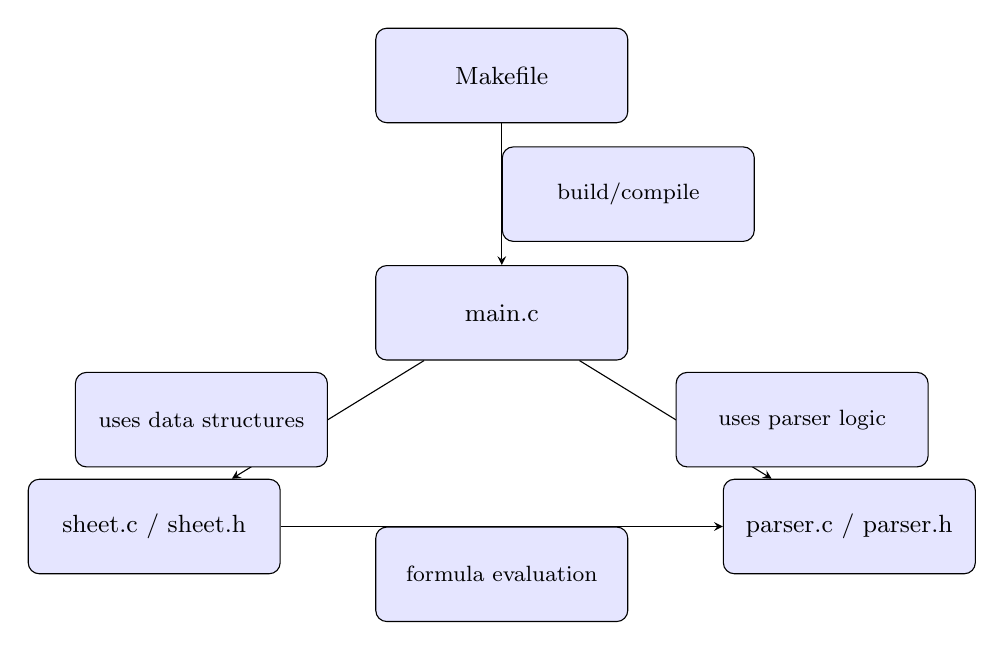
\begin{tikzpicture}[
    >=stealth,
    node distance=2.7cm,
    every node/.style={
        rectangle,
        draw,
        fill=blue!10,
        text centered,
        minimum width=3.2cm,
        minimum height=1.2cm,
        font=\small,
        rounded corners
    }
]

% Nodes
\node (make) {Makefile};
\node (main)  [below=1.8cm of make]        {main.c};
\node (sheet) [below left=1.5cm and 1.2cm of main]  {sheet.c / sheet.h};
\node (parser)[below right=1.5cm and 1.2cm of main] {parser.c / parser.h};

% Edges
\draw[->] (make) -- (main)
    node[midway, right, font=\footnotesize]{build/compile};
\draw[->] (main) -- (sheet)
    node[midway, left, font=\footnotesize]{uses data structures};
\draw[->] (main) -- (parser)
    node[midway, right, font=\footnotesize]{uses parser logic};
\draw[->] (sheet) -- (parser)
    node[midway, below, font=\footnotesize]{formula evaluation};

\end{tikzpicture}
\caption{High-level software structure including the Makefile build process.}
\label{fig:software-structure}
\end{figure}

\subsection{Detailed Software Structure Explanation}
\begin{itemize}[noitemsep]
    \item \textbf{Modularity:}  
    \begin{itemize}[noitemsep]
        \item The clear separation between \texttt{main.c}, \texttt{sheet.c/h}, and \texttt{parser.c/h} ensures that each module can be developed and debugged independently.
        \item Interfaces between modules are well-defined, making it straightforward to integrate additional functionality such as enhanced error reporting or new formula functions.
    \end{itemize}
    \item \textbf{Scalability:}  
    \begin{itemize}[noitemsep]
        \item The DFS-based approach in \texttt{sheet.c} allows the program to efficiently update only those cells that are affected by a change, ensuring performance even with large spreadsheets.
        \item The use of dynamic data structures (like vectors for the adjacency list) supports variable-sized spreadsheets.
    \end{itemize}
    \item \textbf{Extensibility:}  
    \begin{itemize}[noitemsep]
        \item New functions (e.g., additional statistical operations) can be incorporated into the parser with minimal changes to the overall architecture.
        \item Future improvements, such as graphical interfaces or networked collaboration, can build on top of the existing modular design.
    \end{itemize}
    \item \textbf{Error Propagation and Recovery:}  
    \begin{itemize}[noitemsep]
        \item Error codes and messages are managed at the parser level and then propagated to the main application, ensuring that users receive immediate feedback.
        \item In case of critical errors (like circular dependencies), the program is designed to revert changes to maintain consistency.
    \end{itemize}
\end{itemize}

\section{Test Suite and Edge Cases}
We created test cases covering:
\begin{itemize}[noitemsep]
    \item \textbf{Cell assignments:} Direct integer assignments and references (e.g., \texttt{A1=10}, \texttt{B2=A1+5}).
    \item \textbf{Arithmetic expressions:} \texttt{+}, \texttt{-}, \texttt{*}, \texttt{/}, with checks for division by zero.
    \item \textbf{Range-based functions:} \texttt{MIN}, \texttt{MAX}, \texttt{SUM}, \texttt{AVG}, \texttt{STDEV}, including invalid or reversed ranges that trigger errors.
    \item \textbf{\texttt{SLEEP} function:} We handle negative arguments by not actually sleeping, returning the negative integer instead.
    \item \textbf{Circular dependencies:} e.g., \texttt{A1=A1+1} or referencing a range that includes the cell itself.
\end{itemize}
We also tested scenarios where multiple cells in a range contain errors, ensuring the entire range function fails gracefully.

\section{Demo and GitHub}
\begin{itemize}[noitemsep]
    \item \textbf{Demo Video:} \url{https://drive.google.com/file/d/1PUsckK6hrYHW4nh7b5hv7jY0px6P2GeW/view?usp=sharing}
    \item \textbf{GitHub Repository:} \url{https://github.com/2023CS10322/COP290_C_LAB/tree/main}
\end{itemize}

\section{Conclusion}
In this lab, we built a robust spreadsheet program in C that supports formula parsing, selective recalculation, error handling, and circular dependency detection. Our modular design (\texttt{main.c}, \texttt{sheet.c/h}, \texttt{parser.c/h}, and \texttt{Makefile}) allowed us to manage complexity effectively. The program handles a wide variety of edge cases, from invalid ranges to negative sleep times. Overall, this project deepened our understanding of language parsing, data structures, and dependency management, and provided a strong foundation for future enhancements.

\end{document}
